\documentclass[]{AVSSimReportMemo}
\usepackage{AVS}
\usepackage{colortbl}


\newcommand{\ModuleName}{velocityPoint}
\newcommand{\subject}{Guidance Module for Velocity Axis Pointing}
\newcommand{\status}{Initial Version}
\newcommand{\preparer}{M. Cols}
\newcommand{\summary}{Generate the attitude reference to perform a constant pointing towards a Velocity orbit axis}


\begin{document}

\makeCover


%
% enter the revision documentation here
% to add more lines, copy the table entry and the \hline, and paste after the current entry.
%
\pagestyle{empty}
{\renewcommand{\arraystretch}{2}
\noindent
\begin{longtable}{|p{0.5in}|p{4.5in}|p{1.14in}|}
\hline
{\bfseries Rev}: & {\bfseries Change Description} & {\bfseries By} \\
\hline
Draft & initial copy & M. Cols \\
\hline

\end{longtable}
}

\newpage
\setcounter{page}{1}
\pagestyle{fancy}

\tableofcontents
~\\ \hrule ~\\

\section{Module Input and Ouptut}

Table \ref{tab:inputNavTable} shows the input message from the navigation system.
\begin{table}[h!]
	\centering
	\caption{Input Navigation Message}
	\begin{tabular}{|l|l|l|p{3in}|}
		\hline
		\rowcolor{BrickRed}
		\textcolor{white}{Name} & \textcolor{white}{Type} & 
		\textcolor{white}{Length} & 
		\textcolor{white}{Description}  \\ \hline
		$\bm{R}_S$ & double [] & 3 & 
		Position vector of the spacecraft body-point with respect to the inertial frame in inertial frame components 
		($\leftexp{N}{\bm{r}}_{B/N}$) . \\ \hline
		$\bm{v}_S$ & double [] & 3 & 
		Velocity vector of the spacecraft point with respect to the inertial frame in inertial frame components 
		($\leftexp{N}{\bm{v}}_{B/N}$). \\ \hline
	\end{tabular}
	\label{tab:inputNavTable}
\end{table}


Table \ref{tab:inputCelTable} shows the input message from Spice about the main celestial body.
\begin{table}[h!]
	\centering
	\caption{Input Spice Planet Message}
	\begin{tabular}{|l|l|l|p{3in}|}
		\hline
		\rowcolor{BrickRed}
		\textcolor{white}{Name} & \textcolor{white}{Type} & 
		\textcolor{white}{Length} & 
		\textcolor{white}{Description}  \\ \hline
		$\bm{R}_P$  & double [] & 3 & 
		Position vector of the main celestial object with respect to the inertial frame in inertial frame components . \\ \hline
		$\bm{v}_P$  & double [] & 3 & 
		Velocity vector of the main celestial object with respect to the inertial frame in inertial frame components . \\ \hline
	\end{tabular}
	\label{tab:inputCelTable}
\end{table}


Table \ref{tab:outputTable} shows the Attitude Reference output message of the module Velocity Point.
\begin{table}[h!]
	\centering
	\caption{Output Attitude Reference Message}
	\begin{tabular}{|l|l|l|p{3in}|}
		\hline
		\rowcolor{BrickRed}
		\textcolor{white}{Name} & \textcolor{white}{Type} & 
		\textcolor{white}{Length} & 
		\textcolor{white}{Description}  \\ \hline
		$\bm{\sigma}_{R/N}$ & double [] & 3 & 
		MRP attitude set of the reference frame with respect to the reference. \\ \hline
		$\leftexp{N} {\bm{\omega}_{R/N}}$ & double [] & 3 & 
		Angular rate vector of the reference frame with respect to the inertial expressed in inertial frame components. \\ \hline
		$\leftexp{N} {\bm{\dot{\omega}}_{R/N}}$ & double [] & 3 & 
		Angular acceleration vector of the reference frame with respect to the inertial expressed in inertial frame components. \\ \hline
	\end{tabular}
	\label{tab:outputTable}
\end{table}
\newpage

\section{Velocity Frame Definition}
\begin{figure}[htb]
  \centerline{ 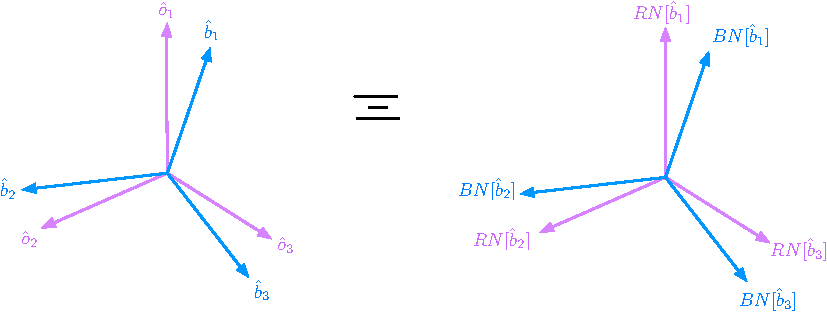
\includegraphics{Figures/Fig2} }
  \caption{Illustration of the planet orbit frames, Hill $\mathcal{H}$ and Velocity $\mathcal{V}$.}
  \label{fig:Fig1}
\end{figure}
The Velocity reference frame takes the spacecraft's orbital plane as the principal one and has origin in the center of the spacecraft. It is defined by the right-handed set of axes $\mathcal{V}:\{ \hat{\bm\imath}_{n}, \hat{\bm\imath}_{v}, \hat{\bm\imath}_{h} \}$, where\par
$\hat {\bm\imath}_{v}$  is tangent to the orbit and parallel to the velocity. \par
$\hat {\bm\imath}_{h}$ is defined normal to the orbital plane in the direction of the angular momentum. \par
$\hat {\bm\imath}_{n}$ completes the right-handed triode.\par

Figure~\ref{fig:Fig1} illustrates the relation between the Hill orbit frame $\mathcal{H}$ and the Velocity orbit frame.  $\mathcal{V}$. These two frames differ by a 3-axis rotation with the angle $-\beta$.  In terms of $\beta$, the DCM to map from $\mathcal{H}$ to $\mathcal{V}$ is given by
\begin{equation}
  \label{eq:VH1}
  [VH] = [M_{3}(-\beta)] = \begin{bmatrix}
    \cos\beta & -\sin\beta & 0 \\
    \sin\beta & \cos\beta &0 \\
    0 & 0 & 1
  \end{bmatrix}
\end{equation}
In terms of the classical set of orbital elements, this DCM can also be expressed as
\begin{equation}
  \label{eq:VH2}
  [VH] = \begin{bmatrix}
    \dfrac{1 + e \cos f}{\sqrt{1+e^{2}+2e \cos f}} & 
    -\dfrac{e \sin f}{\sqrt{1+e^{2}+2e \cos f} }
    & 0 \\
    \dfrac{e \sin f}{\sqrt{1+e^{2}+2e \cos f}}  & \dfrac{1 + e \cos f}{\sqrt{1+e^{2}+2e \cos f}} & 0\\
    0 & 0 & 1
  \end{bmatrix}
\end{equation}

\section{Reference Frame Generation}
\begin{figure}[htb]
  \centerline{ 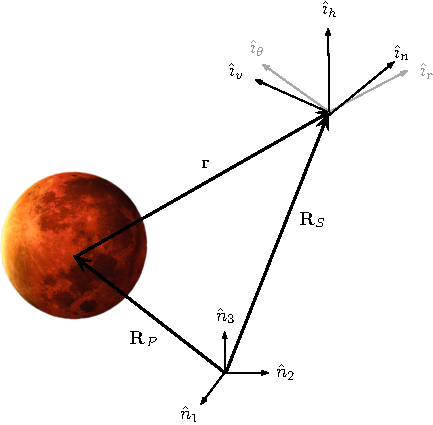
\includegraphics{Figures/Fig1}}
  \caption{Illustration of the inertial frame $\mathcal{N}:\{ \hat{\bm n}_{1}, \hat{\bm n}_{2}, \hat{\bm n}_{3} \}$ and the orbit frames Hill $\mathcal{H}:\{ \hat{\bm\imath}_{r}, \hat{\bm\imath}_{\theta}, \hat{\bm\imath}_{h} \}$ and Velocity $\mathcal{V}:\{ \hat{\bm\imath}_{n}, \hat{\bm\imath}_{v}, \hat{\bm\imath}_{h} \}$ .}
  \label{fig:Fig2}
\end{figure}

In this module, the output reference frame $\mathcal{R}$ is to be aligned with the Velocity reference frame $\mathcal{V}$. Note that the presented technique does not require the planet-fixed  frame to coincide with the inertial frame $\mathcal{N}:\{ \hat{\bm n}_{1}, \hat{\bm n}_{2}, \hat{\bm n}_{3} \}$. Figure 1 illustrates the general situation in which $\bm{R}_{s}$ is the position vector of the spacecraft with respect to the inertial frame and $\bm{R_{p}}$ is the position vector of the  celestial body with respect to the inertial frame as well.

The relative position of the spacecraft with respect to the planet is obtained by simple subtraction:
\begin{equation}
  \label{eq:r}
  \bm r = \bm R_{s} -  \bm R_{p}
\end{equation}
The same methodology is applied to compute the relative velocity vector:
\begin{equation}
  \label{eq:v}
  \bm v = \bm v_{s} -  \bm v_{p}
\end{equation}
Note that the position and velocity vectors of the spacecraft and the celestial body, $\bm{R}_S$,  $\bm{R}_P$,  $\bm{v}_S$ and  $\bm{v}_P$ are the only inputs that this module requires. Having $\bm r$ and $\bm v$, the Velocity frame orientation is completely defined:
\begin{subequations}
  \begin{equation}
  \hat{\bm\imath}_{v} = \frac{\bm v}{v} 
  \end{equation}
  \begin{equation}
  \hat{\bm\imath}_{h} = \frac{\bm{r}\times{\bm{v}}}{rv}
  \end{equation}
  \begin{equation}
  \hat{\bm\imath}_{n} = \hat{\bm\imath}_{v} \times \hat{\bm\imath}_{h}
  \end{equation}
\end{subequations}
And the Direction Cosine Matrix to map from the reference frame to the inertial is obtained:
\begin{equation}
	[RN] =  \begin{bmatrix}
       		\hat{\bm\imath}_{n} \\
		\hat{\bm\imath}_{v} \\ 
		\hat{\bm\imath}_{h}
      \end{bmatrix}
\end{equation}
The corresponding MRP attitude set is computed using the following function from the Rigid Body Kinematics library of Reference~\citenum{schaub}:
$$ [RN] = \textrm{C2MRP}(\bm\sigma_{R/N})$$
\section{Velocity Frame Rate Development}
Next the Velocity frame rate $\dot\beta$ relative to the orbit frame is determined.
Note the following identities from ~\eqref{eq:VH1} and ~\eqref{eq:VH2}: 
\begin{equation}
  \label{eq:tanbeta}
  \tan\beta = \frac{e \sin f}{1 + e \cos f}
\end{equation}
\begin{equation}
  \label{eq:cos2beta}
  \cos^{2}\beta^{} = \frac{(1+e \cos f)^{2}}{1+e^{2}+2 e \cos f}
\end{equation}
Taking the derivative of Eq.~\eqref{eq:tanbeta} yields
\begin{equation}
  \label{eq:dbeta}
  \dot\beta =   \frac{ e (e+\cos f)}{1+e^{2}+2 e \cos f} \dot f
\end{equation}
To find the relative angular acceleration $\ddot\beta$, Eq.~\eqref{eq:dbeta} is differentiated again.
\begin{equation}
  \label{eq:ddbeta}
  \ddot\beta = 
   \frac{e(e+\cos f)}{1+e^{2}+2 e \cos f} \ddot f
   +\frac{
  e  (e^{2}-1)\sin f
  }{
  (1+e^{2}+2 e \cos f)^{2}
  } \dot f^{2}
\end{equation}
The true anomaly rate and acceleration are determined through the standard astrodynamics relations:
\begin{align}
  \dot f &= \frac{h}{r^{2}}
  \\
  \ddot f &= - 2 \frac{\bm v \cdot \hat{\bm\imath}_{r}}{r} \dot f
\end{align}
Following, let us evaluate the Velocity frame angular vectors.  As both the $\mathcal{V}$ and $\mathcal{H}$ frame rotate about the common $\hat{\bm\imath}_{h}$ axis, note that
\begin{equation}
  \label{eq:omegaVN}
  \bm\omega_{V/N} = \bm\omega_{V/H} + \bm\omega_{H/N} = (-\dot\beta + \dot f) \hat{\bm\imath}_{h}
\end{equation}
\begin{equation}
  \label{eq:domegaVN}
  \dot{\bm\omega}_{V/N} = \dot{\bm\omega}_{V/H} + \dot{\bm\omega}_{H/N} = (-\ddot\beta + \ddot f) \hat{\bm\imath}_{h}
\end{equation}

\section{Angular Velocity Descriptions}
Let $\mathcal{R}_{0}$ reference the Velocity orbit frame. Thus, $\bm\omega_{R_{0}/N}$ and $\dot{\bm\omega}_{R_{0}/N}$ correspond to the expressions in ~\eqref{eq:omegaVN} and ~\eqref{eq:domegaVN} respectively.
The angular rate $\bm\omega_{R/N}$ and acceleration $\dot{\bm\omega}_{R/N}$ of the output reference frame $\mathcal{R}$  still need to be computed. 
Since the desired attitude is a fixed-pointing one, $\mathcal{R}$ does not move relative to $\mathcal{R}_{0}$. Thus, the angular velocity of the reference frame happens to be:
\begin{equation}
  \label{eq:omega_R}
  \bm\omega_{R/N} = \bm\omega_{R/R_{0}} + \bm\omega_{R_{0}/N} = \bm\omega_{R_{0}/N} = \frac{1+e \cos f}{1+e^{2} + 2 e \cos f} \dot f \hat{\bm\imath}_{h}
\end{equation}
where $\dot\beta$ and $\dot f$ have been substituted by their corresponding expressions.\newline
Similarly, we find
\begin{equation}
  \label{eq:domega_R}
  \dot{\bm\omega}_{R/N} = \dot{\bm\omega}_{R/R_{0}} + \dot{\bm\omega}_{R_{0}/N} = \dot{\bm\omega}_{R_{0}/N} =
  \left( \frac{1+e\cos f}{1+e^{2}+2 e \cos f} \ddot f
  - \frac{
  e  (e^{2}-1)\sin f
  }{
  (1+e^{2}+2 e \cos f)^{2}
  } \dot f^{2} \right) \hat{\bm\imath}_{h}
\end{equation}
where $\ddot\beta$ and $\ddot f$ have been substituted by their corresponding expressions.

Both $\bm\omega_{R/N}$ and $\bm{\dot\omega}_{R/N} $ need to be expressed in the inertial frame $N$. \newline
Given 
\begin{subequations}
\begin{equation}
\leftexp{R}{\bm \omega_{R/N} } = 
      \begin{bmatrix}
       0\\ 0 \\ \dot{f}-\dot\beta
      \end{bmatrix}
\end{equation}
\begin{equation}
 \leftexp{R}{\bm{\dot{\omega}}_{R/N}  } = 
      \begin{bmatrix}
       0\\ 0 \\ \ddot{f}-\ddot\beta
      \end{bmatrix}
\end{equation}
\end{subequations}
Then, 
\begin{subequations}
\begin{equation}
	\leftexp{N} {\bm{\omega}_{R/N}} =  [NR] \textrm{ }\leftexp{R} {\bm{\omega}_{R/N} }
\end{equation}
\begin{equation}
	\leftexp{N} {\bm{\dot{\omega}}_{R/N} }=[NR]\textrm{ }\leftexp{R} {\bm{\dot{\omega}}_{R/N}}
\end{equation}
\end{subequations}
Where $ [NR] = [RN]^T$.

\bibliographystyle{unsrt}
\bibliography{references}

\end{document}
